%!TEX encoding = UTF-8 Unicode
\documentclass[master,korean,final]{cbnu-ecs}

% kaist.cls 에서는 기본으로 dhucs, ifpdf, graphicx 패키지가 로드됩니다.
% 추가로 필요한 패키지가 있다면 주석을 풀고 적어넣으십시오,
%\usepackage{...}
%

%\usepackage{kotex}
\usepackage{multirow}
\usepackage{varwidth}
\usepackage{amsmath}
\usepackage{indentfirst}
\usepackage{algorithm,algpseudocode}
\usepackage{booktabs}
\usepackage{longtable}

%\renewcommand\tablename{표}
%\renewcommand\figurename{그림}

\newtheorem{theorem}{Theorem}	

% @command title 논문 제목
% @options [default: (none)]
% - korean: 한글제목 | english: 영문제목
\title[korean]{선분 카메라쌍 알고리즘을 이용한 사각형 특징의 기하학적 자세 추정을 통한 Factor Graph 기반 비주얼 SLAM}
\title[english]{Factor Graph based Visual SLAM with Geometric Pose Estimation of a Rectangle Feature using Coupled Line Camera Algorithm}

\author[korean] {이}{재 민}
\author[english]{Lee}{Jae-Min}

\advisor[major]{박 찬 식}{Chan sik Park}{signed}

\department{RO}

% @command studentid 학번
\studentid{2014298010}

% 논문제출일
\submitdate{2016}{6}{3}

% @command approvaldate 지도교수논문승인일
% @param   year,month,day 연,월,일 순으로 입력
\approvaldate{2016}{6}{3}

% @command refereedate 심사위원논문심사일
% @param   year,month,day 연,월,일 순으로 입력
\refereedate{2016}{6}{3}

% @command gradyear 졸업년도
\gradyear{2016}{8}

% 본문 시작
\begin{document}

% 목차 (Table of Contents) 생성
\tableofcontents
% 그림목차 (List of Figures) 생성
\listoffigures
% 표목차 (List of Tables) 생성
\listoftables
% 영문초록 (abstract)
\begin{abstract}
Modern networks are large-scale, composed of many layers with tens of thousands of devices. 
Cloud computing data centers and multi-layered transport networks are 
examples of such networks.
\ldots
\end{abstract}





% 위의 세 종류의 목차는 한꺼번에 다음 명령으로 생성할 수도 있습니다.
%\makecontents

\pagenumbering{arabic}

\chapter{서론}

%\begin{figure}[!ht]
%  \centering
%	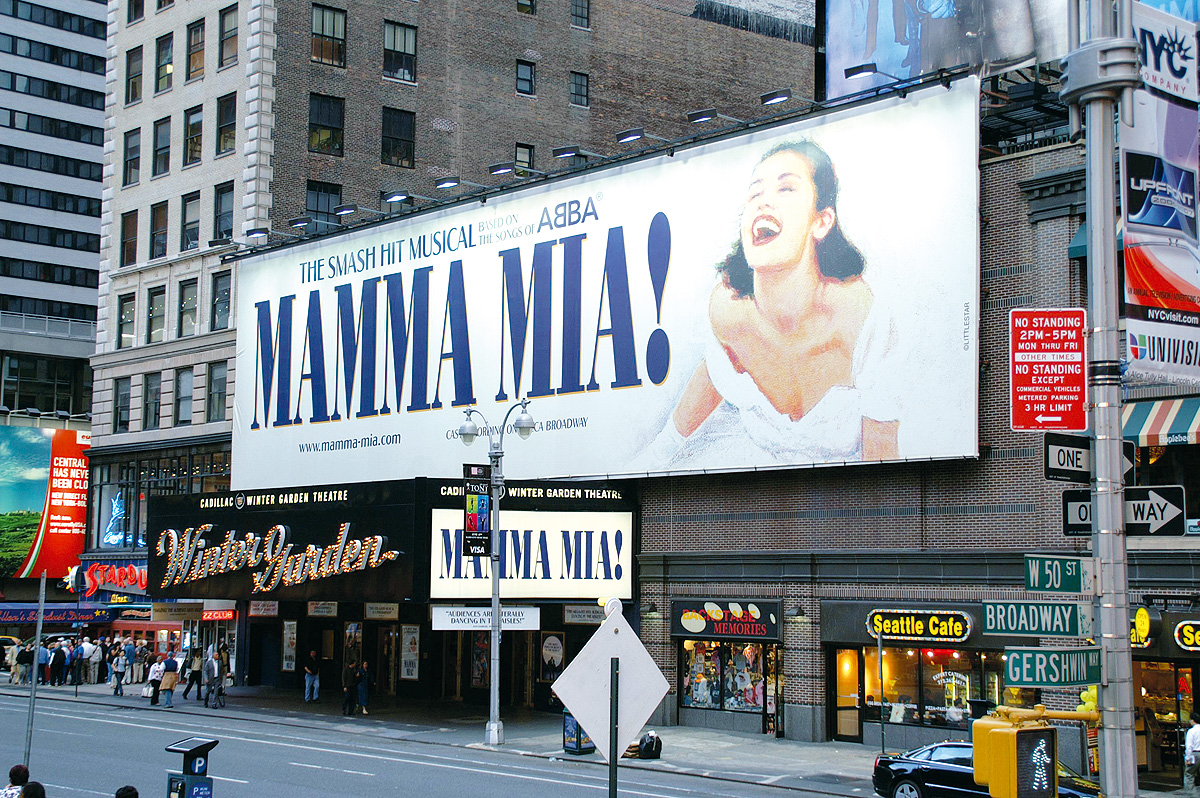
\includegraphics[width=360px]{img/BroadwayPlayers_01.jpg}
%  \caption{A picture of the same gull looking the other way!}
%\end{figure}

%\fontsize{11}{20.5}\selectfont

\section{연구 배경}
자율 이동 로봇의 성공적인 임무 수행을 위해서는 주변 환경의 정보를 정합하고 자신의 위치를 파악하여 목표로의 접근을 위한 구동을 결정할 수 있어야 한다. 이 때 화성 탐사선, 재난 구조 로봇, 탄광 탐사로봇과 같이 사전에 정보가 주어지지 않은 환경에 놓인 로봇은 취득한 환경정보를 이용하여 스스로 지도를 작성하고 그 위의 자신의 위치를 추정하며 임무를 수행하여야 한다. 이러한 기술을 SLAM(Simultaneous Localization and Mapping)이라 하고 1986년 미국의 IEEE Robotics and Automation Conference에서 확률론적으로 문제에 접근하는 방안에 대한 토의를 가진 이후 이를 기반으로 연구가 계속되고 있다\cite{Durrant2006}. 확률론으로 SLAM문제를 수식화하여 계산하기 위해 전통적으로 Extended Kalman Filter\cite{Dissanayake2000}, Unscented Kalman Filter\cite{Martinez2005}, Extended Information Filter\cite{Thrun2003}, Rao-Blackwellized Particle Filter\cite{Montemerlo2002}등의 recursive bayesian filtering기술이 응용되었다. 이후 SLAM문제를 Belief Network, Markov Random Field등의 그래프 모델로 표현하고 그래프 최적화 기술을 이용하여 해결하고자 하는 시도가 이어졌고\cite{Kummerle2011}, 
현재까지 많은 연구자들이 이 접근법을 바탕으로 SLAM기술의 계산 복잡도, loop closure, 동적으로 변하는 환경 등에 대한 문제를 강인한 특징 추출 방식 제안 및 센서 처리 방식 개선, 지도 표현 방식 변경과 같은 다양한 방법으로 해결하고자 하는 노력이 이어지고 있다.\\
알려지지 않은 환경의 정보를 취득하기 위해 어떤 센서를 사용할 것인지 결정하는 것은 SLAM기술의 구제척인 형태와 성능을 크게 좌우한다. 센서로는 거리정보 기반의 LiDAR(Light Detection and Ranging)센서와 Sonar(Sound Navigation and Ranging)센서, RF(Radio Frequency) 또는 자기장을 이용한 인공 표식 인식 센서 그리고 카메라 등이 이용될 수 있다. 그러나 자율 이동 로봇이 임무를 수행하기 위한 환경 중 우주나 재해환경, 접근 불가 지역과 같이 사람의 접근과 활동의 제약이 존재하는 환경에서 인공 표식을 사전에 설치하여 SLAM에 활용하는 것은 굉장히 제한적일 수 밖에 없다. 따라서 SLAM에 관련된 많은 연구와 적용 사례들은 주어진 환경을 직접 추출할 수 있는 거리-방향 센서를 사용하여 문제를 정의하며 해결하고 있다. 그 중 자율 이동 로봇의 응용으로 가장 많이 연구되고 있는 두 센서는 LiDAR와 카메라로, 단일 센서를 이용한 연구는 물론 복수의 센서 또는 융합 센서 시스템을 구성하여 SLAM문제를 해결하는 연구도 활발하게 진행되어 왔다.\\
LiDAR는 센서로 부터 송출된 적외선의 Time-of-Flight를 응용하여 2차원 혹은 3차원 환경에 대한 거리 정보를 취득하는 능동형 센서이다. 충분히 강한 출력의 광원이 사용된다면 조명에 강인하고 일정한 검출 시간과 성능을 보장받을 수 있는 장점이 있으나 고정밀기계장치를 이용하여 충격에 민감하고 가격이 고가이다. 또한 점군으로 표현된 환경에 대한 거리정보는 취득 영역의 부피에 비해 비교적 적은 수 이고, 신호 세기 등 거리 이외의 정보는 취급이 어렵거나 사용이 제한적이기 때문에 데이터의 정보량은 비교적 적다고 할 수 있다. 카메라는 외부의 광원에서 발해져 직접 투사되거나 주변 물체에 반사되어 들어온 가시광선 근방의 전자기파에 대한 정보를 취득하는 감응형 센서이다. 주변 광원의 상태에 따라 사용에 제약을 받을 수 있으나 저렴한 가격에 고밀도의 환경정보를 취득할 수 있는 장점이 있다.
연산에 사용되는 로봇의 컴퓨터 혹은 연구용 워크스테이션의 성능이 높아지면서 보다 방대한 자료를 빠르게 처리할 수 있게 되어, 최근에는 가격이 비싸고 용도가 제한적인 LiDAR센서 대신 카메라를 이용하는 SLAM기술의 연구가 각광을 받고 있다. 또한 두 센서의 장점을 살려 융합 시스템을 구축, 활용하는 방법도 제시되어 있다\cite{Newman2006}.

\section{관련 연구}
\cite{Davison2007}

\subsection{사각형 특징을 활용한 종래 연구}

%%%%%%%%%%%%%%%%%%%%%%%%%%%%%%%%%%%%%%%%%%%%%%%%%%%%%%%%%%%%%%%%%%%%%%%%%%%%%%%%%%%%%%%%%%%%%%%%%%%%%%%%%%%%%%%%%%%%%%%%%%%%%%%%%%%
%%%%%%%%%%%%%%%%%%%%%%%%%%%%%%%%%%%%%%%%%%%%%%%%%%%%%%%%%%%%%%%%%%%%%%%%%%%%%%%%%%%%%%%%%%%%%%%%%%%%%%%%%%%%%%%%%%%%%%%%%%%%%%%%%%%
%%%%%%%%%%%%%%%%%%%%%%%%%%%%%%%%%%%%%%%%%%%%%%%%%%%%%%%%%%%%%%%%%%%%%%%%%%%%%%%%%%%%%%%%%%%%%%%%%%%%%%%%%%%%%%%%%%%%%%%%%%%%%%%%%%%
\chapter{사각형 특징 추출(segmentation)}
%%%%%%%%%%%%%%%%%%%%%%%%%%%%%%%%%%%%%%%%%%%%%%%%%%%%%%%%%%%%%%%%%%%%%%%%%%%%%%%%%%%%%%%%%%%%%%%%%%%%%%%%%%%%%%%%%%%%%%%%%%%%%%%%%%%
%%%%%%%%%%%%%%%%%%%%%%%%%%%%%%%%%%%%%%%%%%%%%%%%%%%%%%%%%%%%%%%%%%%%%%%%%%%%%%%%%%%%%%%%%%%%%%%%%%%%%%%%%%%%%%%%%%%%%%%%%%%%%%%%%%%
%%%%%%%%%%%%%%%%%%%%%%%%%%%%%%%%%%%%%%%%%%%%%%%%%%%%%%%%%%%%%%%%%%%%%%%%%%%%%%%%%%%%%%%%%%%%%%%%%%%%%%%%%%%%%%%%%%%%%%%%%%%%%%%%%%%
\chapter{사각형 특징 기반 Visual SLAM}
\section{자세 추정을 위한 사각형 복원 방법}
\subsection{선분 카메라쌍 방법을 이용한 사각형 복원 방법}
\subsection{3차원 자세 추정을 위한 스테레오 카메라 기반의 선분카메라쌍 방법}
\section{FactorGraphSLAM}
\subsection{}
%%%%%%%%%%%%%%%%%%%%%%%%%%%%%%%%%%%%%%%%%%%%%%%%%%%%%%%%%%%%%%%%%%%%%%%%%%%%%%%%%%%%%%%%%%%%%%%%%%%%%%%%%%%%%%%%%%%%%%%%%%%%%%%%%%%
%%%%%%%%%%%%%%%%%%%%%%%%%%%%%%%%%%%%%%%%%%%%%%%%%%%%%%%%%%%%%%%%%%%%%%%%%%%%%%%%%%%%%%%%%%%%%%%%%%%%%%%%%%%%%%%%%%%%%%%%%%%%%%%%%%%
%%%%%%%%%%%%%%%%%%%%%%%%%%%%%%%%%%%%%%%%%%%%%%%%%%%%%%%%%%%%%%%%%%%%%%%%%%%%%%%%%%%%%%%%%%%%%%%%%%%%%%%%%%%%%%%%%%%%%%%%%%%%%%%%%%%
\chapter{Data Association}
%%%%%%%%%%%%%%%%%%%%%%%%%%%%%%%%%%%%%%%%%%%%%%%%%%%%%%%%%%%%%%%%%%%%%%%%%%%%%%%%%%%%%%%%%%%%%%%%%%%%%%%%%%%%%%%%%%%%%%%%%%%%%%%%%%%
%%%%%%%%%%%%%%%%%%%%%%%%%%%%%%%%%%%%%%%%%%%%%%%%%%%%%%%%%%%%%%%%%%%%%%%%%%%%%%%%%%%%%%%%%%%%%%%%%%%%%%%%%%%%%%%%%%%%%%%%%%%%%%%%%%%
%%%%%%%%%%%%%%%%%%%%%%%%%%%%%%%%%%%%%%%%%%%%%%%%%%%%%%%%%%%%%%%%%%%%%%%%%%%%%%%%%%%%%%%%%%%%%%%%%%%%%%%%%%%%%%%%%%%%%%%%%%%%%%%%%%%
\chapter{Feature Desctiption}
%%%%%%%%%%%%%%%%%%%%%%%%%%%%%%%%%%%%%%%%%%%%%%%%%%%%%%%%%%%%%%%%%%%%%%%%%%%%%%%%%%%%%%%%%%%%%%%%%%%%%%%%%%%%%%%%%%%%%%%%%%%%%%%%%%%
%%%%%%%%%%%%%%%%%%%%%%%%%%%%%%%%%%%%%%%%%%%%%%%%%%%%%%%%%%%%%%%%%%%%%%%%%%%%%%%%%%%%%%%%%%%%%%%%%%%%%%%%%%%%%%%%%%%%%%%%%%%%%%%%%%%
%%%%%%%%%%%%%%%%%%%%%%%%%%%%%%%%%%%%%%%%%%%%%%%%%%%%%%%%%%%%%%%%%%%%%%%%%%%%%%%%%%%%%%%%%%%%%%%%%%%%%%%%%%%%%%%%%%%%%%%%%%%%%%%%%%%
\chapter{실험결과}
\section{CLC Pose estimation validation}
\section{Room/indoor robot test}
\section{Outdoor(Campus) test}
\section{Public Dataset}
\section{Descriptor Test}
%%%%%%%%%%%%%%%%%%%%%%%%%%%%%%%%%%%%%%%%%%%%%%%%%%%%%%%%%%%%%%%%%%%%%%%%%%%%%%%%%%%%%%%%%%%%%%%%%%%%%%%%%%%%%%%%%%%%%%%%%%%%%%%%%%%
%%%%%%%%%%%%%%%%%%%%%%%%%%%%%%%%%%%%%%%%%%%%%%%%%%%%%%%%%%%%%%%%%%%%%%%%%%%%%%%%%%%%%%%%%%%%%%%%%%%%%%%%%%%%%%%%%%%%%%%%%%%%%%%%%%%
%%%%%%%%%%%%%%%%%%%%%%%%%%%%%%%%%%%%%%%%%%%%%%%%%%%%%%%%%%%%%%%%%%%%%%%%%%%%%%%%%%%%%%%%%%%%%%%%%%%%%%%%%%%%%%%%%%%%%%%%%%%%%%%%%%%
\chapter{결론}


%%%%%%%%%%%%%%%%%%%%%%%%%%%%%%%%%%%%%%%%%%%%%%%%%%%%%%%%%%%%%%%%%%%%%%%%%%%%%%%%%%%%%%%%%%%%%%%%%%%%%%%%%%%%%%%%%%%%%%%%%%%%%%%%%%%
%%%%%%%%%%%%%%%%%%%%%%%%%%%%%%%%%%%%%%%%%%%%%%%%%%%%%%%%%%%%%%%%%%%%%%%%%%%%%%%%%%%%%%%%%%%%%%%%%%%%%%%%%%%%%%%%%%%%%%%%%%%%%%%%%%%
%%%%%%%%%%%%%%%%%%%%%%%%%%%%%%%%%%%%%%%%%%%%%%%%%%%%%%%%%%%%%%%%%%%%%%%%%%%%%%%%%%%%%%%%%%%%%%%%%%%%%%%%%%%%%%%%%%%%%%%%%%%%%%%%%%%
\chapter{실험결과}

본 논문에서 제안하는 방법의 타당성을 평가하기위해 몇가지 실험을 통해 입증한다. \\
asdasda\\
asdasd\\
asdasda
sdas

%%%%%%%%%%%%%%%%%%%%%%%%%%%%%%%%%%%%%%%%%%%%%%%%%%%%%%%%%%%%%%%%%%%%%%%%%%%%%%%%%%%%%%%%%%%%%%%%%%%%%%%%%%%%%%%%%%%%%%%%%%%%%%%%%%%
%%%%%%%%%%%%%%%%%%%%%%%%%%%%%%%%%%%%%%%%%%%%%%%%%%%%%%%%%%%%%%%%%%%%%%%%%%%%%%%%%%%%%%%%%%%%%%%%%%%%%%%%%%%%%%%%%%%%%%%%%%%%%%%%%%%
%%%%%%%%%%%%%%%%%%%%%%%%%%%%%%%%%%%%%%%%%%%%%%%%%%%%%%%%%%%%%%%%%%%%%%%%%%%%%%%%%%%%%%%%%%%%%%%%%%%%%%%%%%%%%%%%%%%%%%%%%%%%%%%%%%%
\chapter{결론}

dd


%%%%%%%%%%%%%%%%%%%%%%%%%%%%%%%%%%%%%%%%%%%%%%%%%%%%%%%%%%%%%%%%%%%%%%%%%%%%%%%%%%%%%%%%%%%%%%%%%%%%%%%%%%%%%%%%%%%%%%%%%%%%%%%%%%%
%%%%%%%%%%%%%%%%%%%%%%%%%%%%%%%%%%%%%%%%%%%%%%%%%%%%%%%%%%%%%%%%%%%%%%%%%%%%%%%%%%%%%%%%%%%%%%%%%%%%%%%%%%%%%%%%%%%%%%%%%%%%%%%%%%%
%%%%%%%%%%%%%%%%%%%%%%%%%%%%%%%%%%%%%%%%%%%%%%%%%%%%%%%%%%%%%%%%%%%%%%%%%%%%%%%%%%%%%%%%%%%%%%%%%%%%%%%%%%%%%%%%%%%%%%%%%%%%%%%%%%%
% references section

% can use a bibliography generated by BibTeX as a .bbl file
% BibTeX documentation can be easily obtained at:
% http://www.ctan.org/tex-archive/biblio/bibtex/contrib/doc/
% The IEEEtran BibTeX style support page is at:
% http://www.michaelshell.org/tex/ieeetran/bibtex/
%\bibliographystyle{IEEEtran}
% argument is your BibTeX string definitions and bibliography database(s)
%\bibliography{IEEEabrv,../bib/paper}
%
% <OR> manually copy in the resultant .bbl file
% set second argument of \begin to the number of references
% (used to reserve space for the reference number labels box)

\bibliographystyle{IEEEtran}%...는 bst 파일의 이름(확장자 없이)
\bibliography{ThesisBibTeX.bib}%...는 bib 파일의 이름(확장자 없이)
%\begin{thebibliography}{1}
%\bibitem{greenberg}
%A. Greenberg, J. Hamilton, D.A. Maltz, and P. Patel,
%\emph{The cost of a Cloud: Research Problems in Data Center Networks},
%ACM SIGCOMM Computer Communication Review (CCR), 
%Vol. 39, No. 1, pp. 68-73, January 2009.
%
%\bibitem{wallin}
%S. Wallin, V. Leijon, 
%\emph{Telecom Network and Service Management: An Operator Survey}, 
%MMNS, 2009.
%
%\bibitem{hscalability}
%Wikipedia, \emph{Horizontal Scalability},
%\url{http://en.wikipedia.org/wiki/Scalability#Scale_horizontally_.28scale_out.29}
%
%\end{thebibliography}


\chapter*{감사의 글}

감사의 글을 적으시면 되겠습니다.
감사합니다.sssss

\begin{flushright}
\vspace{1cm}
이재민 배상
\end{flushright}

\end{document}


